%%
%% This is file `sample-acmlarge.tex',
%% generated with the docstrip utility.
%%
%% The original source files were:
%%
%% samples.dtx  (with options: `acmlarge')
%% 
%% IMPORTANT NOTICE:
%% 
%% For the copyright see the source file.
%% 
%% Any modified versions of this file must be renamed
%% with new filenames distinct from sample-acmlarge.tex.
%% 
%% For distribution of the original source see the terms
%% for copying and modification in the file samples.dtx.
%% 
%% This generated file may be distributed as long as the
%% original source files, as listed above, are part of the
%% same distribution. (The sources need not necessarily be
%% in the same archive or directory.)
%%
%%
%% Commands for TeXCount
%TC:macro \cite [option:text,text]
%TC:macro \citep [option:text,text]
%TC:macro \citet [option:text,text]
%TC:envir table 0 1
%TC:envir table* 0 1
%TC:envir tabular [ignore] word
%TC:envir displaymath 0 word
%TC:envir math 0 word
%TC:envir comment 0 0
%%
%%
%% The first command in your LaTeX source must be the \documentclass command.
\documentclass[acmlarge]{acmart}
\usepackage{listings}
\lstset{language=Go,
  basicstyle=\ttfamily\scriptsize,
  keywordstyle=\color{blue}\ttfamily,
  stringstyle=\color{red}\ttfamily,
  commentstyle=\color{green}\ttfamily}
%%ss[STYLE]{acmart}
%% \BibTeX command to typeset BibTeX logo in the docs
\AtBeginDocument{%
  \providecommand\BibTeX{{%
    \normalfont B\kern-0.5em{\scshape i\kern-0.25em b}\kern-0.8em\TeX}}}

%% Rights management information.  This information is sent to you
%% when you complete the rights form.  These commands have SAMPLE
%% values in them; it is your responsibility as an author to replace
%% the commands and values with those provided to you when you
%% complete the rights form.
\setcopyright{acmcopyright}
\copyrightyear{2022}
\acmYear{2022}
\acmDOI{}


%%
%% These commands are for a JOURNAL article.
\acmJournal{POMACS}
\acmVolume{37}
\acmNumber{4}
\acmArticle{7}
\acmMonth{8}

%%
%% Submission ID.
%% Use this when submitting an article to a sponsored event. You'll
%% receive a unique submission ID from the organizers
%% of the event, and this ID should be used as the parameter to this command.
%%\acmSubmissionID{123-A56-BU3}

%%
%% The majority of ACM publications use numbered citations and
%% references.  The command \citestyle{authoryear} switches to the
%% "author year" style.
%%
%% If you are preparing content for an event
%% sponsored by ACM SIGGRAPH, you must use the "author year" style of
%% citations and references.
%% Uncommenting
%% the next command will enable that style.
%%\citestyle{acmauthoryear}

%%
%% end of the preamble, start of the body of the document source.
\begin{document}

%%
%% The "title" command has an optional parameter,
%% allowing the author to define a "short title" to be used in page headers.
\title{Paper Reading of \textit{PerfScope: Practical Online Server Performance Bug Inference in Production Cloud Computing Infrastructures}}

%%
%% The "author" command and its associated commands are used to define
%% the authors and their affiliations.
%% Of note is the shared affiliation of the first two authors, and the
%% "authornote" and "authornotemark" commands
%% used to denote shared contribution to the research.
\author{Yiwei Yang}
\email{yangyw@shanghaitech.edu.cn}
\orcid{0000-0001-8011-5868}
\affiliation{
  \institution{ShanghaiTech University}
  \streetaddress{1 R.D. Zhongke}
  \city{Shanghai}
  \state{Shanghai}
  \country{China}
  \postcode{21210}
}

%%
%% By default, the full list of authors will be used in the page
%% headers. Often, this list is too long, and will overlap
%% other information printed in the page headers. This command allows
%% the author to define a more concise list
%% of authors' names for this purpose.
\renewcommand{\shortauthors}{Yiwei Yang}

%%
%% The abstract is a short summary of the work to be presented in the
%% article.
\begin{abstract}
  The paper \cite{dean2014perfscope} introduce a performance triggered bug identification paradigm. It would have dig into the syscalls and jvm calls to trace all the frequent closed system call episodes. The cause of performance bugs may be overflow cause by while loop, which can be reduced by trace aware abnormal execution triggered dynamic static analysis by signature extraction. Each function signature represents a group of closed frequent system call experiences (for example, sys write, *, and sys read). When a performance fault occurs in production, we extract the closed frequent system call episodes from the anomalous execution units and use the function signatures to map those episodes back to a limited list of probable buggy functions. We then give those identified functions a ranking depending on the degree of abnormality seen in those frequent system call occurrences. 
  \begin{figure}[htbp]
    \centering
    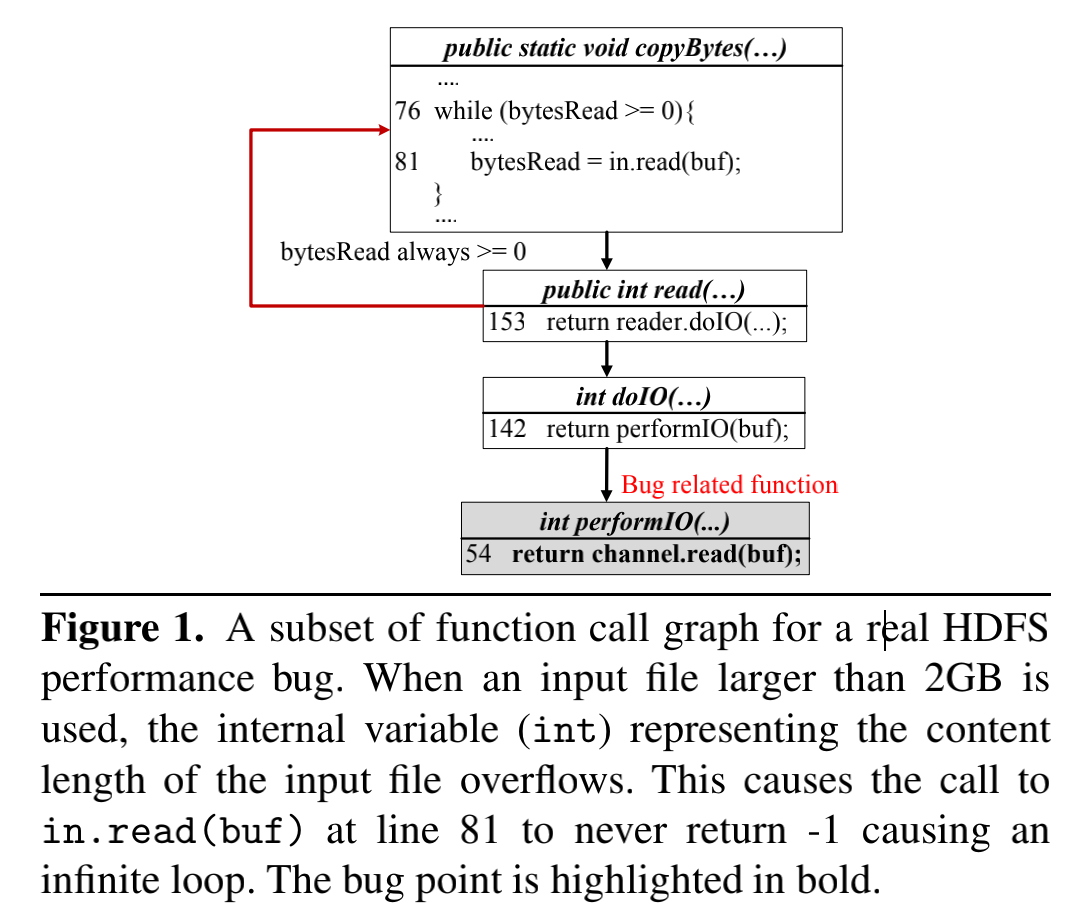
\includegraphics[width=10cm]{./bug.png}
  \end{figure}
 \end{abstract}

%%
%% The code below is generated by the tool at http://dl.acm.org/ccs.cfm.
%% Please copy and paste the code instead of the example below.
%%
\begin{CCSXML}
  <ccs2012>
  <concept>
  <concept_id>10010520.10010553.10010562</concept_id>
  <concept_desc>Distributed System~Peer to Peer System</concept_desc>
  <concept_significance>500</concept_significance>
  </concept>
  </ccs2012>
\end{CCSXML}

\ccsdesc[500]{Distributed System~Bug identification}

%%
%% Keywords. The author(s) should pick words that accurately describe
%% the work being presented. Separate the keywords with commas.
\keywords{Performace Bug. System Call Tracing}


%%
%% This command processes the author and affiliation and title
%% information and builds the first part of the formatted document.
\maketitle
\section{Strong point of the document}

\subsection{Novel Abnormal Execution Unit identifications}
The process is monitored by identifying the abnormal execution unit, which apples the top-down logic to get the syscall appearance vector for each execution unit.  The [sys write, sys read, sys poll] syntax is used for the system call appearance vector in this scenario. [1,1,0] and [0,1,1], respectively, would represent the system call appearance vectors for the two execution units. Because two comparable execution units could output varying numbers of the same system call type due to dynamic runtime environments, we chose the system call appearance vector as the clustering feature vector to achieve robust grouping. The bug function list generation is for Function Episode $FE_{AEU}$. The analysis is whether the FE exists and increases in incorrect order. The root related function can be traced back using FSM.
\subsection{Efficiency in Bug Inference}
The memtable mishandling problem's root of cause can be easily found to help the developer fix the bug. Some dynamic tools only trigger bugs and do not give solving hints like fuzzing.
\section{Weak point of the document}
\subsection{The bug finding is too one-directional}
The bugs found are mostly caused by the gettimeofday and assertion in timestamp, reload cache cassedra bugs.
\subsection{FSM explosion}
The FSM construction requires limited syscalls and do AEU propagation. The storage to store FSM is space consuming, I ponder whether it can be compressed.
\section{Possible refinement}
\subsection{A better system level info can be leveraged}
Other than LLTng for syscall parameter, buffer and return code plus pid and TCB be recorded and thus construct the $FM_{AEU}$ and FSM. However, these state can now be observed by eBPF which is faster than syscall observation.
\subsection{A stronger program analysis tool can be applied}
The algorithm is pretty straightforward that do simple vector clustering and cast analysis for pattern matched root of case like 90\% bug appearance loop and assert operations.
\bibliographystyle{ACM-Reference-Format}
\bibliography{perfScope_practical_online_server_performance_bug_inference_in_production_cloud_computing_infrastructures}
\end{document}
\endinput
%%
%% End of file `sample-acmlarge.tex'.
